\section{Introduction}
\label{sec:introduction}
\IEEEPARstart{T}{iny Tapeout} is a multi project chip platform that makes it easier and cheaper to get application specific integrated circuit (ASIC) designs manufactured.

Open source tools and process design kits (PDKs~\cite{pdk}) are used so no restrictive licenses or non disclosure agreements (NDAs) are required. As the tools run on remote cloud servers no software needs to be installed locally on the user's machine. As long as the template structure is followed, however, Tiny Tapeout can support the use of proprietary tools.

Each Tiny Tapeout ASIC production run has around 400 open source designs multiplexed to 24 general purpose input/output (GPIO) pins. After manufacture the resulting chip is mounted to a demonstration board for ease of testing. Each chip contains a copy of every design which can be selected and tested in turn.

At the same time each participant submits documentation for their design, which is used to create a printable datasheet~\cite{datasheet} alongside an online project index at \url{TinyTapeout.com/runs/}~\cite{tinytapeoutruns}. The datasheet helps participants explore other designs on the chip in addition to their own.

By separating the cost of area on a silicon wafer and the finished physical chip, the Tiny Tapeout participant group is able to share the cost of chip packaging and of circuit board manufacture while still being able to test and measure all the designs on the chip. For use in educational settings it is possible for multiple students to submit individual designs while sharing the finished chips and circuit boards, reducing the cost still further.

Each Tiny Tapeout tile (Fig.~\ref{fig:render_cells_in_use}) is approximately $\qty{160} \times \qty{100}{\micro\meter\squared}$. This provides enough room for around \qty{1000} logic gates when built upon the SkyWater \qty{130}{\nm} open source PDK. Multiple tiles can be interconnected to enable larger designs, while analog and mixed signal support is on the roadmap for the next shuttle.

The first~\cite{firstshuttle} Tiny Tapeout production run, which was provided as a free and experimental effort with a total of \qty{152} designs, was submitted to the seventh Google sponsored~\cite{googlesponsored} lottery based multi project wafer (MPW) shuttle in September 2022.
The next four shuttles combined a total of \qty{582} designs, all sponsored by and manufactured through the Efabless~\cite{efabless} chipIgnite MPW service on the SkyWater \qty{130}{\nm} process. Table~\ref{tab:tinytapeout} shows a summary of all Tiny Tapeout shuttle runs to date.

Individuals submitting designs to Tiny Tapeout tend to self identify as hobbyists, students, and teachers, as shown in Fig.~\ref{fig:TT04_submitters}.

\begin{figure}[!t]
\centering
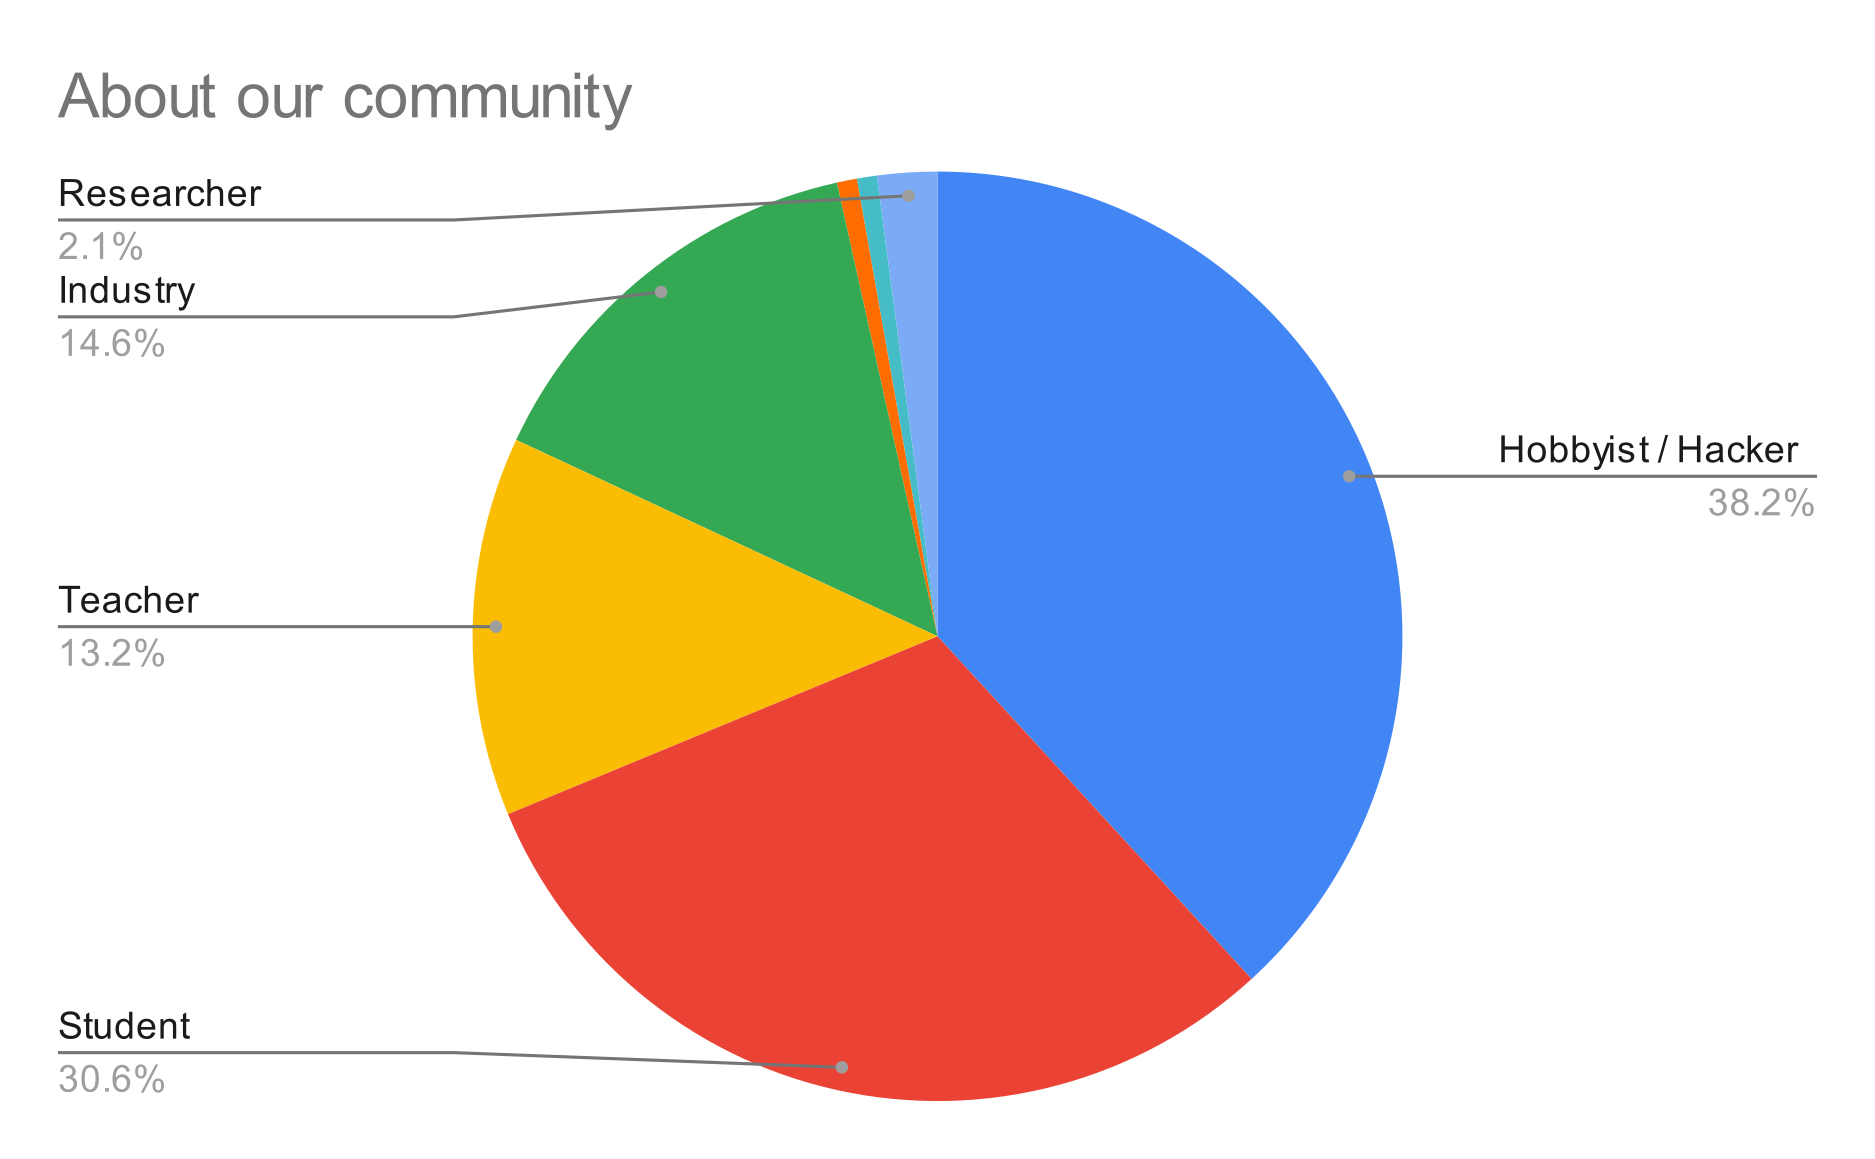
\includegraphics[width=\columnwidth]{./Figs/about our community pie chart.png}
\caption{Tiny Tapeout 4 participant self identification.}
\label{fig:TT04_submitters}
\end{figure}

The remainder of this paper will detail the Tiny Tapeout submission flow, multiplexer evolution, circuit board design, the results of post production silicon testing, and the project's next steps.

\begin{table*}[!t]
\centering
\caption{Tiny Tapeout shuttle summary}
\label{tab:tinytapeout}
\begin{tabularx}{\textwidth}{@{}l *{9}{X}@{}}
\toprule
\textbf{Run} & \textbf{Launched} & \textbf{Shuttle} & \textbf{Designs} & \textbf{Delivery date} & \textbf{Architecture} & \textbf{Number of IOs} & \textbf{IO bandwidth} & \textbf{Analog support} \\
\midrule
TT01 & 2022-08-17  & MPW7  & 152 & n/a        & Scan chain                & 16 & \qty{5}{\kHz}    & no  \\
TT02 & 2022-11-09  & 2211Q & 165 & 2024-01-30 & Scan chain                & 16 & \qty{5}{\kHz}    & no  \\
TT03 & 2023-03-01  & 2304C & 249 & 2024-02-28 & Scan chain inverted clock & 16 & \qty{10}{\kHz}    & no  \\
TT04 & 2023-07-01  & 2309  & 143 & 2024-04-15 & Mux                       & 26 & \qty{50}{\MHz}   & no  \\
TT05 & 2023-09-11  & 2311  & 174 & 2024-05-12 & Split Mux                 & 26 & \qty{50}{\MHz}   & no  \\
TT06 & 2024-02-01  & 2404  & TBD & 2024-11-30 & Split Mux                 & 38 & \qty{50}{\MHz}   & yes \\
\bottomrule
\end{tabularx}
\end{table*}

\begin{figure}[!t]
\centering
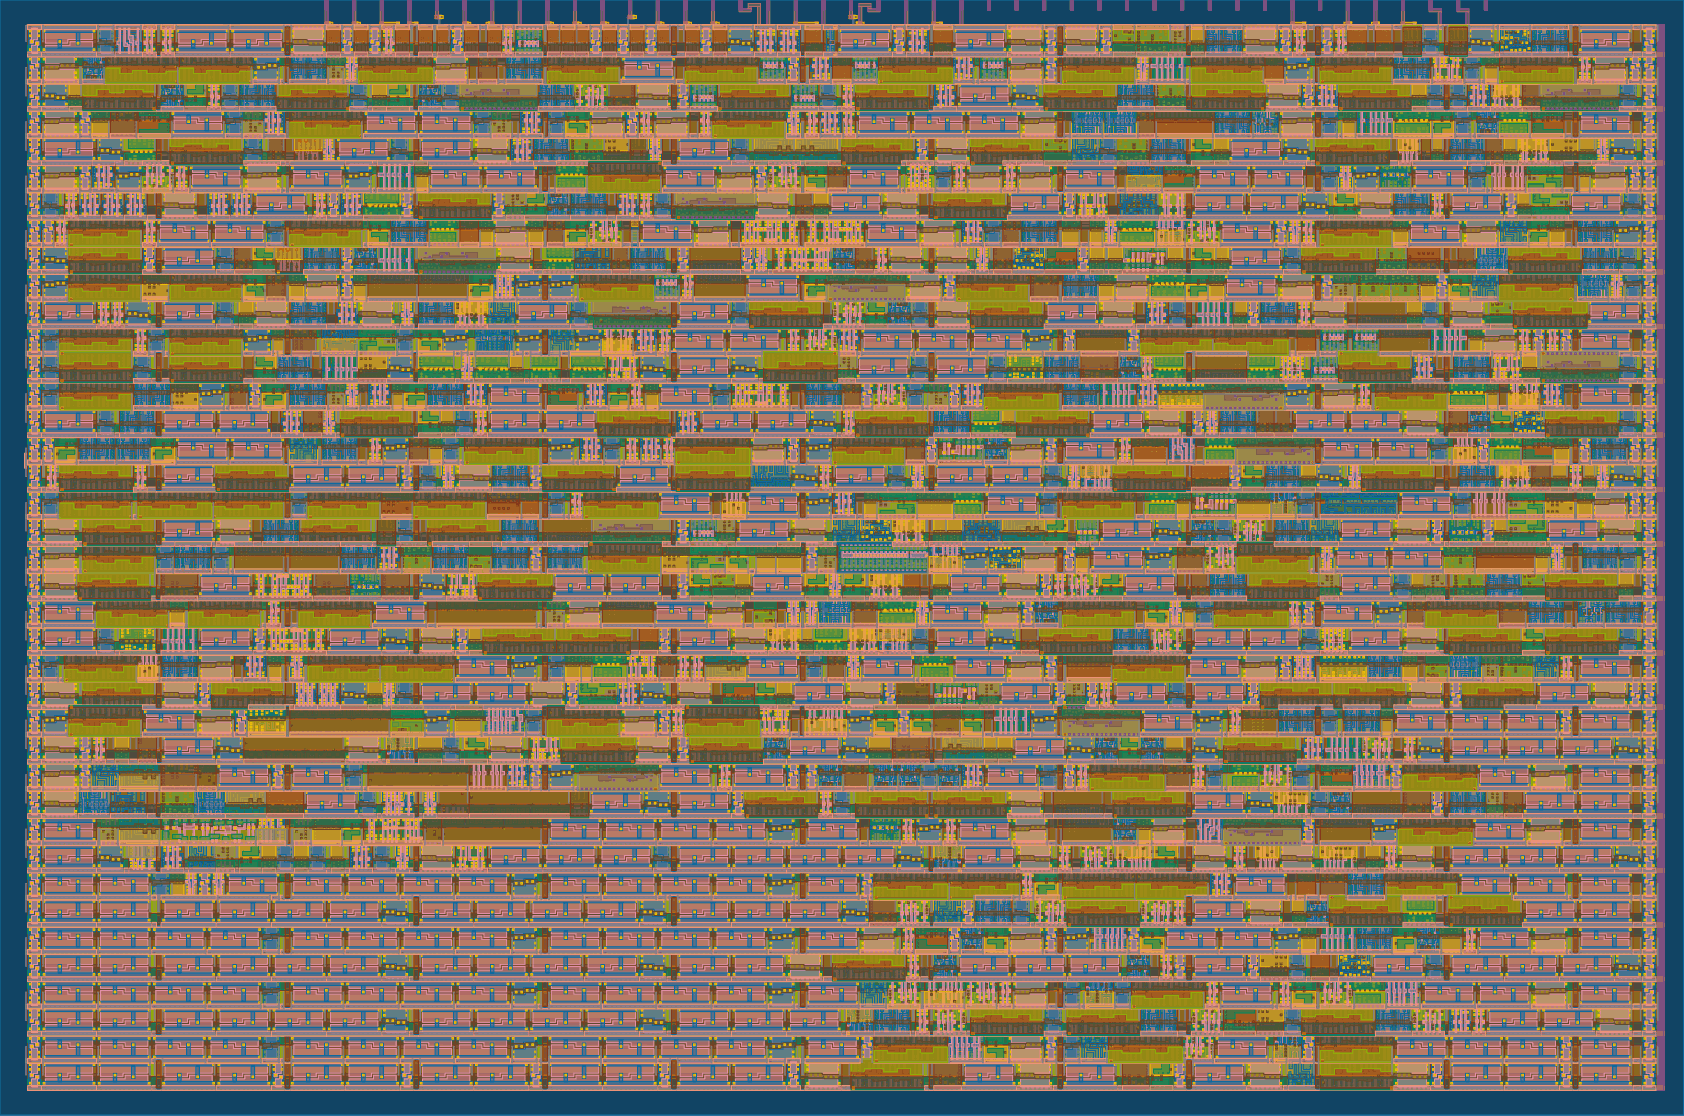
\includegraphics[width=\columnwidth]{./Figs/gh action gds layout.png}
\caption{A 2-D render of a single Tiny Tapeout tile.}
\label{fig:render_cells_in_use}
\end{figure}
